\documentclass[12pt]{article}

\usepackage{fontawesome}
\usepackage{hyperref}
\usepackage{xurl}
\usepackage{graphicx}
\usepackage{float}
\usepackage[tagged, highstructure]{accessibility}
\usepackage{bookmark}
\usepackage{enumitem}

\hypersetup{
    colorlinks=false,
    pdfborder={0 0 0},
    pdftitle={Big Data},
    pdfauthor={Adrianna Holden-Gouveia},
    pdfsubject={Advanced Data - Lab Assignment},
    pdflang={en-US},
    pdfkeywords={big data, machine learning, Khan Academy, tutorials, Python}
}

% Configure PDF bookmarks for navigation
\bookmarksetup{
    numbered,
    open,
}

% Configure list spacing for better accessibility
\setlist{nosep}



\title{Big Data}
\author{
        Adrianna Holden-Gouveia \\
        Website: \href{https://aholdengouveia.name}{aholdengouveia.name}\\ 
        \date{\vspace{-5ex}}
        %Email: \href{mailto:admin@aholdengouveia.name}{admin@aholdengouveia.name} \\
%        \faLinkedin{: aholdengouveia} \\
        \faGithub {: aholdengouveia} \\
        %\faTwitter {: aholdengouveia} \\
        }

%S\date{\today}


\begin{document}    

\maketitle

%\begin{abstract}
%This is a template for Linux Administration Lab work
%\end{abstract}
%\tableofcontents


\section*{Accessibility Notice}
This document is also available in HTML format at:

Link: \href{https://aholdengouveia.name/AdvData/labs/wk10bigdata.html}{\textbf{\nolinkurl{https://aholdengouveia.name/AdvData/labs/wk10bigdata.html}}}

The HTML version provides enhanced accessibility features including keyboard navigation, screen reader support, responsive design, dark mode support, and high contrast options.

\section*{Request}
\noindent\textbf{Request:} DATA-2058\\
\textbf{Requested by:} Head of the data team\\
\textbf{Data:} Your database, and your list of new data from the Database Matchmaking lab

\section*{Background}
Everyone at the company keeps talking about big data. Before anyone spends money on it, your manager wants to know whether the company's data actually counts as big data, what new data would be worth collecting, how it would be collected and checked, and where it should all be stored. You'll also do some training in data analysis and machine learning, so the team has a shared starting point.

\section*{Learning Outcomes}
By the end of this lab, you will be able to:
\begin{itemize}
    \item Assess whether a data set is big data, using the 3 Vs and other characteristics
    \item Plan how to collect and verify new data that would grow a data set, and decide whether it's worth it
    \item Recommend a data warehouse, data lake, or data lakehouse for a company's data, and justify it
    \item Evaluate tutorials for quality, length, and who they are best suited for
\end{itemize}

\section*{Lab Instructions}
Use your own data set and company. Books are my example data only.

\subsection*{Screenshots}
Several parts of this lab ask for a screenshot. Each screenshot should have your name, term, and year.  One of the easiest ways to do that is make a text document with your name and term/year on your computer and save it to use all term. Any screenshots that don't include this information won't be counted.

\begin{figure}[H]
    \centerline{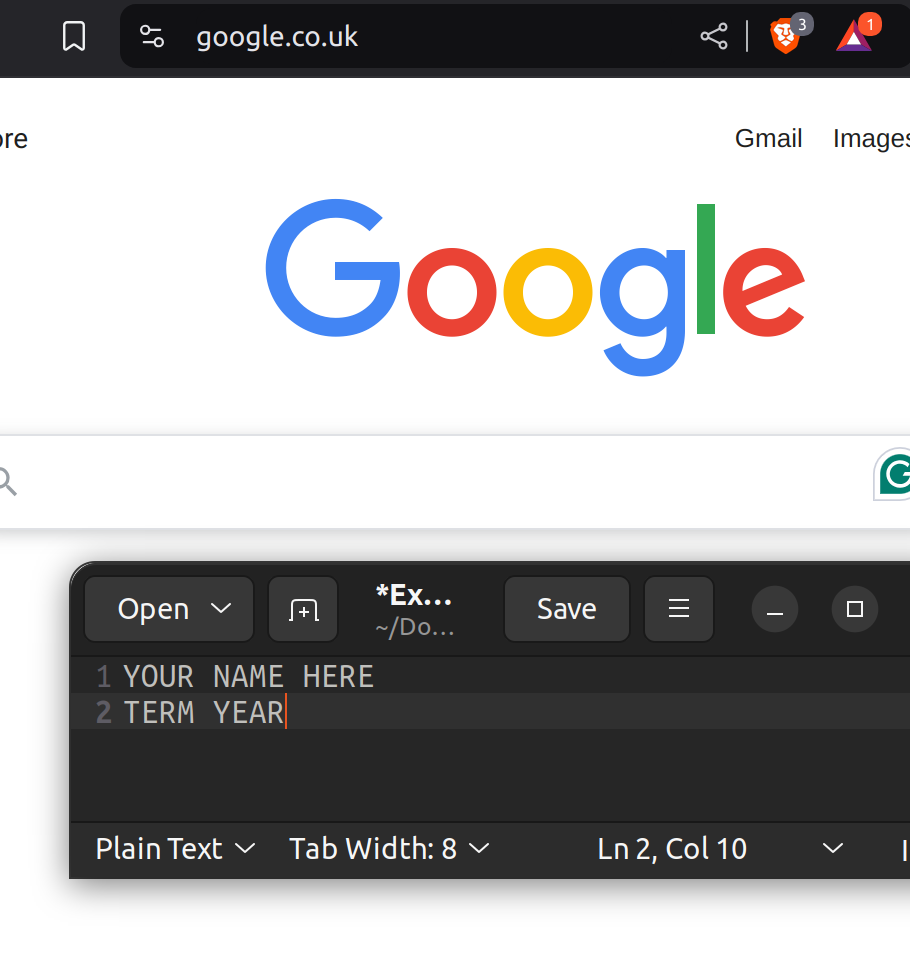
\includegraphics[scale=.2]{ExampleScreenshot.png}}
    \caption{This is an image of what each of your screenshots should look like}
    \alt{Example screenshot: a web browser showing the Google home page, with a small text editor window in front of it that says YOUR NAME HERE and TERM YEAR}
\end{figure}

\subsection*{Part 1: Data Analysis Tutorial}
Go through the Khan Academy Data Analysis 101 tutorial (linked under Resources).
\begin{enumerate}
    \item Take a screenshot of your completed problems.
    \item What did you think of this tutorial? Why?
    \item Would you recommend this tutorial to others? Why or why not?
    \item What do you think was missing from this tutorial?
\end{enumerate}

\subsection*{Part 2: Choose Your Own Tutorial}
Pick one free tutorial from the course list on GitHub (linked under Resources). If you already have some Python skill, you can do Kaggle's Intro to Machine Learning course instead. There's a wide variety of options at different skill levels and lengths. If you pick a long one, you don't need to finish it, just do enough to get an idea of how it goes.
\begin{enumerate}
    \item Take a screenshot of your progress in the tutorial.
    \item Which tutorial did you pick, how long is it, and how much of it did you do?
    \item Would you recommend it to others? Why or why not? Note any skills someone would need first.
    \item What was missing, or what skills do you wish you'd had to understand it better?
\end{enumerate}

\subsection*{Part 3: Is Your Data Big Data?}
The topic page describes the 3 Vs of big data, volume, velocity, and variety, along with veracity, variability, and value. For each one, describe your data set, using specific numbers where you can, such as the number of rows, how often new data arrives, and the types of data. Then explain whether your data counts as big data, and why or why not.

\subsection*{Part 4: Data Collection Plan}
Plan how your company could grow its data. Follow the sample data collection plan (linked under Resources). Start from your list of new data from the Database Matchmaking lab, and pick at least 3 new kinds of data. For each one, explain:
\begin{enumerate}
    \item What you would collect, and why: what decision would it help someone at your company make?
    \item How it would be collected, and how often.
    \item How much there would be, as a rough estimate with your working, such as rows per day or per year.
    \item How you would verify it's accurate. For example, comparing totals against another system, or using a left join to find rows with no match.
    \item Whether you need permission to collect it, such as consent for personal data.
    \item Which of the Vs it adds to: volume, velocity, or variety.
\end{enumerate}
Then answer two questions about your plan as a whole:
\begin{enumerate}
    \item Would your data be big data with this new data added? Why or why not? If your data was already big data, which V would become the biggest challenge?
    \item Would collecting this data be worth it for your company? More data isn't always more value, so say which new data is worth collecting first, and why.
\end{enumerate}

\subsection*{Part 5: Storage Recommendation}
Recommend whether your company should store its data, including the new data from your plan, in a data warehouse, a data lake, or a data lakehouse. Explain your choice in one or two paragraphs, using what you found in Parts 3 and 4. Use the topic page and at least one other source, cited with a link and checked with the CRAAP test (linked under Resources).

\section*{Acceptance Criteria}
This request is done when:
\begin{itemize}
    \item Both tutorials have screenshots and answers to all the questions
    \item All 6 characteristics are described for your data, with specific numbers where possible
    \item You've explained whether your data is big data, and why
    \item Your data collection plan covers at least 3 new kinds of data, each with what and why, how it's collected, how much, how it's verified, permission, and which V it adds
    \item You've explained whether your plan would make it big data, and which new data is worth collecting first
    \item Your storage recommendation is justified using your own data and at least one cited source
    \item Every screenshot follows the screenshot rules
\end{itemize}

\section*{Deliverables}
One file that includes Parts 1 to 5.

Audience: the head of the data team.

\section*{Resources}
References, a video, a PowerPoint and some notes are available at my website
Link: \href{https://www.aholdengouveia.name/AdvData/BigData.html}{\textbf{\nolinkurl{https://www.aholdengouveia.name/AdvData/BigData.html}}}

Sample data collection plan, for Part 4
Link: \href{https://www.aholdengouveia.name/AdvData/labs/SampleDataCollectionPlan.txt}{\textbf{\nolinkurl{https://www.aholdengouveia.name/AdvData/labs/SampleDataCollectionPlan.txt}}}

Khan Academy Data Analysis 101, for Part 1
Link: \href{https://www.khanacademy.org/computing/ap-computer-science-principles/data-analysis-101}{\textbf{\nolinkurl{https://www.khanacademy.org/computing/ap-computer-science-principles/data-analysis-101}}}

Course list on GitHub, for Part 2
Link: \href{https://github.com/SkalskiP/courses}{\textbf{\nolinkurl{https://github.com/SkalskiP/courses}}}

Kaggle Intro to Machine Learning, for Part 2 if you know some Python
Link: \href{https://www.kaggle.com/learn/intro-to-machine-learning}{\textbf{\nolinkurl{https://www.kaggle.com/learn/intro-to-machine-learning}}}

The CRAAP test, for checking your sources
Link: \href{https://web.archive.org/web/20250814000638/https://guides.lib.uchicago.edu/c.php?g=1241077&p=9082343}{\textbf{\nolinkurl{https://web.archive.org/web/20250814000638/https://guides.lib.uchicago.edu/c.php?g=1241077&p=9082343}}}

My guide to evaluating sources
Link: \href{https://www.aholdengouveia.name/Howtos/Sourceeval/sourceEvaluation.html}{\textbf{\nolinkurl{https://www.aholdengouveia.name/Howtos/Sourceeval/sourceEvaluation.html}}}

\end{document}